% ---
% JAVA ME EMBEDDED
%
% ---

% TODO
% - refatorar os <tab> por <spaces> e wrap do texto, utilizando emacs
% - revisão do texto em .pdf

\chapter{Java ME Embedded}

Este capítulo tem como objetivo demonstrar a plataforma \textit{Java Embedded} 
- \textit{Java ME Embedded}.

\section{Instalação}

A plataforma de prototipagem deve estar operacional com o sistema operacional 
\textit{Linux} e a plataforma \textit{Java 8}, no caso de estudo a plataforma 
\textit{Raspberry PI B+}. A figura \ref{fig:java-me/configuracao} apresenta as 
configurações do sistema em estudo.

\begin{figure}[H]
    \centering
    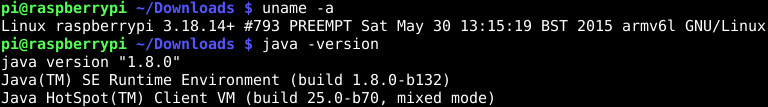
\includegraphics[width=0.7\linewidth]{figuras/java/configuracao}
    \caption{Configuração do Sistema}
    \label{fig:java-me/configuracao}
\end{figure}

Para a plataforma de prototipagem é necessário a instalação do pacote 
\textit{Oracle Java ME Embedded 8.1 for Raspberry Pi Model B (ARM11/Linux)}, 
necessário ter uma conta no site da \textit{Oracle} para realizar o 
\textit{download}.

Transfira o arquivo 
\verb|oracle-jmee-8-1-rr-raspberrypi-linux-bin.zip| do sistema operacional 
principal para o dispositivo remoto, basta utilizar o comando \textit{SCP}:

\verb|scp </path/from/file> <user>@<address>:/path/to/destination|

Descompacte o arquivo, basta utilizar o comando \textit{UNZIP}:

\verb|unzip <file>|

Aplique a permissão 777 para os diretórios \textit{appdb} e \textit{bin}, basta 
utilizar o comando \textit{CHMOD}:

\verb|chmod -R 777 appdb bin|

\subsection{Pacote Oracle Java ME Embedded ZIP}

O pacote \textit{Oracle Java ME Embedded ZIP} consiste de cinco diretórios:

\begin{itemize}
    
    \item /appdb: este diretório é utilizado pela plataforma de prototipagem e 
    contém as bibliotecas interna do \textit{Java};
    
    \item /bin: este diretório é utilizado pela plataforma de prototipagem para 
    instalar, executar e remover as aplicações \textit{IMlets}, possui os 
    executáveis, \textit{scripts} e o arquivo de configuração do 
    \textit{Java} \verb|jwc_properties.ini|;
    
    \item /legal: este diretório contém a documentação de licença;
    
    \item /lib: este diretório é utilizado no processo de compilação dos 
    \textit{IMlets}, contém os arquivos necessários para a execução do 
    \textit{Developer Agent};
    
    \item /util: este diretório possui o arquivo \verb|proxy.jar|, requerido 
    para a comunicação entre plataforma de prototipagem e \textit{Desktop} 
    através do \textit{Developer Agent}.
    
\end{itemize}

No \textit{NetBeans IDE 8} ative o \textit{Java ME}, instale os arquivos 
\textit{Oracle Java ME SDK 8.1} e \textit{plugin} \textit{Oracle Java ME SDK 
8.1 Plugins for NetBeans 8}, necessário ter uma conta no site da 
\textit{Oracle} para realizar o \textit{download}. O \textit{Oracle Java ME SDK 
8.1} somente possui versão para o sistema operacional \textit{Windows x86/64}.

\subsection{Desenvolvimento}

O processo de desenvolvimento inicia pela codificação da aplicação, em seguida 
seu aprimoramento pela documentação da Interfaces de Programação de Aplicação - 
\textit{Application Programming Interfaces} (\textit{APIs}), quando concluído é 
exercitado pelo emulador e finalmente a implantação no dispositivo.

O exemplo aplicado trata-se de um gerador de Modulação por Largura de Pulso - 
\textit{Pulse-Width Modulation} (\textit{PWM}) para a produção de sinais para 
fins como transmitir informações em baixo nível para outros dispositivos.

\subsubsection{Codificação}

A aplicação consiste de um \textit{software} \textit{IMlet}, uma classe na qual 
estende \newline
 \verb|javax.microedition.midlet.MIDlet| e implementa dois métodos:

\begin{itemize}
    
    \item \verb|startApp()|: sinaliza a aplicação a transição para o estado 
    Ativo.
    
    \item \verb|destroyApp()|: sinaliza a aplicação a transição para o estado 
    Destruído.
    
\end{itemize}

O código final é apresentado abaixo:
\newpage
\begin{verbatim}
// JavaMEExample.java
package ufabc;

import java.io.IOException;
import javax.microedition.midlet.MIDlet;
import jdk.dio.DeviceManager;
import jdk.dio.pwm.PWMChannel;

public class JavaMEExample extends MIDlet {
    
    PWMChannel channel;
    
    @Override
    public void startApp() {
        System.out.println("Início da Aplicação");
        try {
            channel = (PWMChannel) DeviceManager.open(18);
            channel.setPulsePeriod(1000000);
            channel.generate(500000, 10);
        } catch (IOException ex) {
        }
    }

    @Override
    public void destroyApp(boolean unconditional) {
        try {
            channel.close();
        } catch (IOException ex) {
        }
        System.out.println("Encerramento da Aplicação");
    }
}
\end{verbatim}

O acesso aos periféricos são realizados através da permissão da \textit{API} pela requisição do \verb|jdk.dio.DeviceMgmtPermission| em 
Descritor de Aplicações - \textit{Application Descriptor}, a figura 
\ref{fig:java-me/application-descriptor} apresenta as permissões para o exemplo 
acima.

\begin{figure}[H]
    \centering
    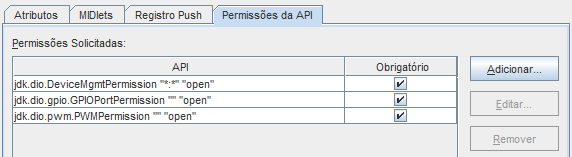
\includegraphics[width=0.7\linewidth]{figuras/java/java-me-application-descriptor.png}
    \caption{Descritor de Aplicações}
    \label{fig:java-me/application-descriptor}
\end{figure}

\subsubsection{Device I/O API}

A \textit{Device I/O API} (Entrada/Saída - \textit{Input/Output}) (Interface de Programação de Aplicação - \textit{Application Programming Interface}) provê uma biblioteca para o acesso aos periféricos de 
baixo nível em sistema embarcados através da plataforma \textit{Java}. Sua 
utilização possui a mesma simplicidade das demais bibliotecas do pacote 
\textit{Java}, pois basta a consulta ao \textit{javadoc} e aplicar as 
implementações. A figura \ref{fig:java-me/java-me-javadoc-deviceioapi} apresenta a estrutura \textit{javadoc} dos pacotes do \textit{Device I/O API}.

\begin{figure}[H]
	\centering
	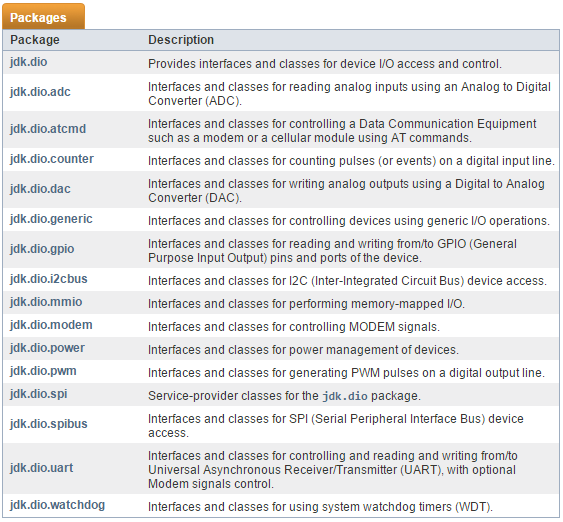
\includegraphics[width=0.7\linewidth]{figuras/java/java-me-javadoc-deviceioapi.png}
	\caption{Pacotes do Device I/O API}
	\label{fig:java-me/java-me-javadoc-deviceioapi}
\end{figure}

\subsubsection{Emulador}

O \textit{Java ME SDK 8 Embedded} incorpora uma emulador de dispositivos para a 
visualização e controle dos periféricos e recursos encontrados nos 
dispositivos, na figura \ref{fig:java-me/emulator} apresenta a tela inicial do 
emulador e na figura \ref{fig:java-me/pwm} a visualização da execução do 
aplicativo de \textit{PWM}.

\begin{figure}[H]
    \centering
    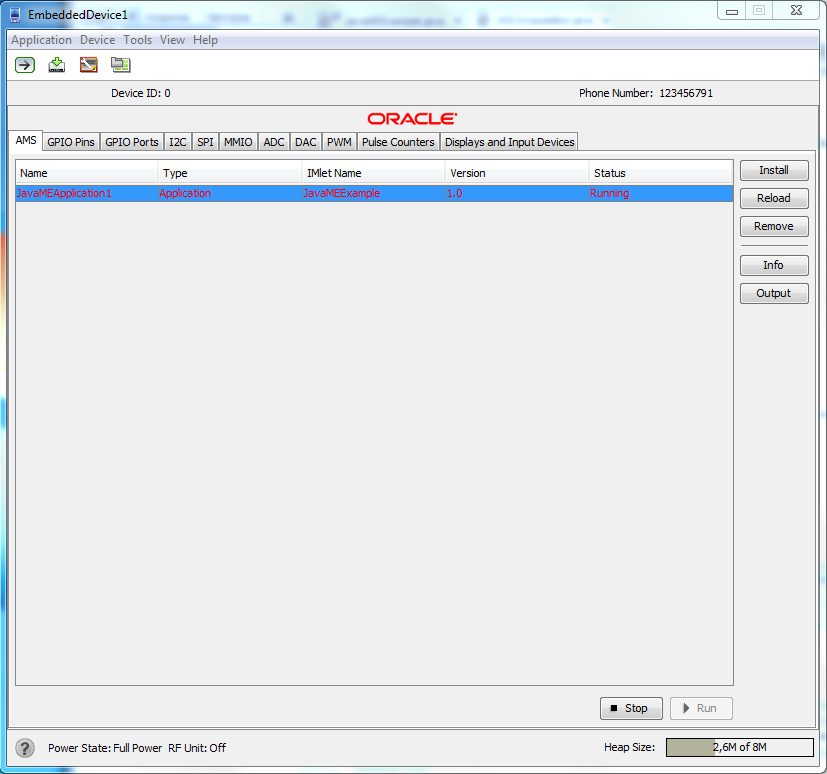
\includegraphics[width=0.7\linewidth]{figuras/java/java-me-emulator.png}
    \caption{Emulador}
    \label{fig:java-me/emulator}
\end{figure}

\begin{figure}[H]
    \centering
    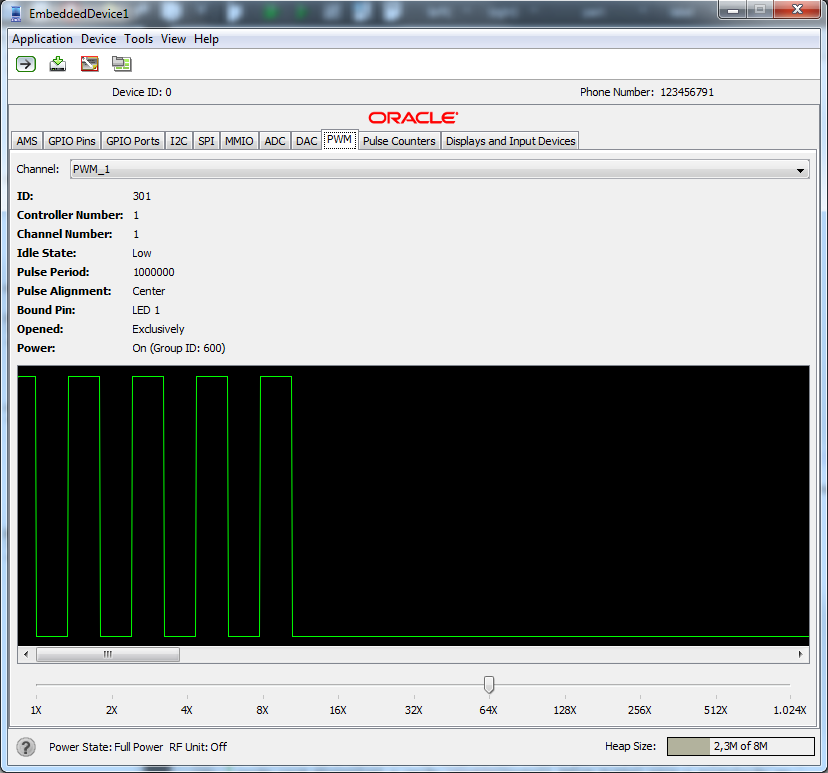
\includegraphics[width=0.7\linewidth]{figuras/java/java-me-pwm.png}
    \caption{Sinal PWM}
    \label{fig:java-me/pwm}
\end{figure}

Diversas ferramentas são encontradas no emulador, tais como controle de 
conectividade, visualização da saída padrão e gerador de eventos externos, na 
figura \ref{fig:java-me/external-events-generator} apresenta a tela para gerar 
eventos para o periférico Entrada/Saída de Propósito Geral - \textit{General 
Purpose Input/Output} (\textit{GPIO}).

\begin{figure}[H]
    \centering
    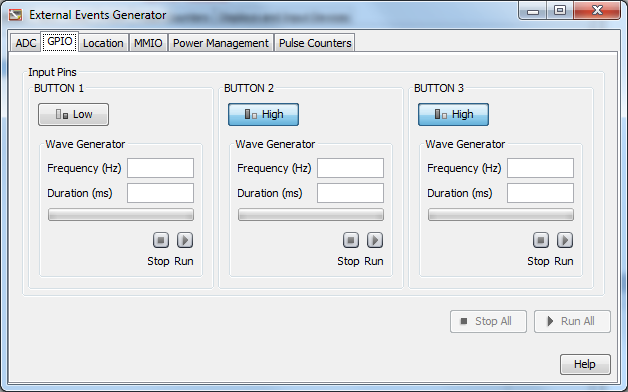
\includegraphics[width=0.7\linewidth]{figuras/java/java-me-external-events-generator.png}
    \caption{Emulador}
    \label{fig:java-me/external-events-generator}
\end{figure}

\subsubsection{Implantação}

O processo de implantação requer a execução do \textit{script} 
\verb|usertest.sh| para a inicialização do \textit{Java} no dispositivo remoto.
No projeto escolha o dispositivo externo para a plataforma, como na figura 
\ref{fig:java-me/plataform}.

\begin{figure}[H]
    \centering
    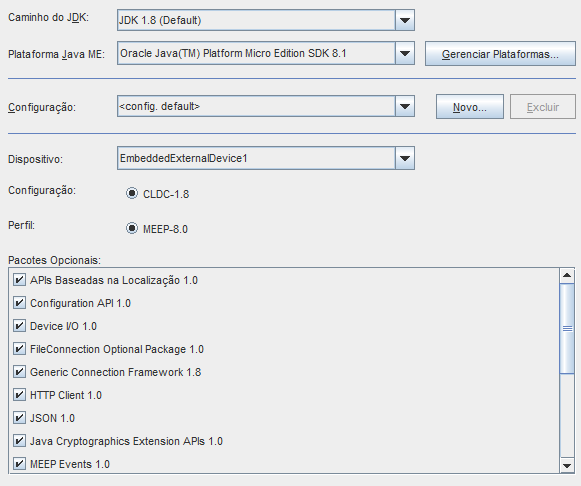
\includegraphics[width=0.7\linewidth]{figuras/java/java-me-plataform.png}
    \caption{Dispositivo Embarcado Externo}
    \label{fig:java-me/plataform}
\end{figure}

O emulador será conectado ao dispositivo remoto para a execução da aplicação, 
porém será disponível a opção \textit{Install IMlet Suite} para a instalação no 
dispositivo.

Outra opção é transferir a aplicação Descritor da Aplicação \textit{Java} - 
\textit{Java Application Descriptor} (\textit{JAD}) para o dispositivo remoto e 
executar o \textit{script} \verb|installMidlet.sh| e \verb|runSuite.sh|.

\section{Aplicações para a Internet das Coisas}

O interfaceamento com periféricos de baixo nível permite a utilização de uma 
gama de fontes de dados, tais como sensores e atuadores. Esses dados podem 
serem combinados com outros dispositivos embarcados.

\section{Resultados}

Os resultados demonstram a visão na qual a plataforma \textit{Java ME Embedded} 
contribui para o desenvolvimento de aplicações destinadas a \textit{Internet} 
das Coisas - \textit{Internet of Things} (\textit{IoT}).

\subsection{Positivos}

\begin{itemize}
    
    \item Permite uma abstração dos periféricos de baixo nível, sem a 
    necessidade de endereços e estruturas de \textit{bits} através da 
    \textit{Device I/O API};
    
    \item O Emulador auxilia no desenvolvimento de aplicações, por 
    disponibilizar uma variedade de interfaces de \textit{hardware}.
    
\end{itemize}

\subsection{Negativos}

\begin{itemize}
    
    \item O \textit{Java ME 8 SDK} não possui uma versão para o sistema 
    operacional \textit{Linux}, o que dificulta durante o ciclo de 
    desenvolvimento;
    
    \item A aplicação necessidade ser inicializada pelo Sistema Operacional, 
    para aplicações autônomas.
    
\end{itemize}
